\documentclass[lettersize,journal]{IEEEtran}
\usepackage{amsmath,amsfonts}
\usepackage{algorithmic}
\usepackage{algorithm}
\usepackage{array}
\usepackage[caption=false,font=normalsize,labelfont=sf,textfont=sf]{subfig}
\usepackage{textcomp}
\usepackage{stfloats}
\usepackage{url}
\usepackage{verbatim}
\usepackage{graphicx}
\usepackage{cite}

%\usepackage{float}
%\usepackage{multirow}
%\usepackage{tabularx}
%\usepackage{authblk}
\usepackage{booktabs}
\hyphenation{op-tical net-works semi-conduc-tor IEEE-Xplore}
% updated with editorial comments 8/9/2021

\begin{document}
\title{Defending Byzantine Attacks in Ensemble Federated Learning: A Reputation-based Phishing Approach}
\author{Beibei~Li,~\IEEEmembership{Member,~IEEE,}
        Peiran~Wang,~\IEEEmembership{Student Member,~IEEE,}
        Qinglei~Kong,~\IEEEmembership{Member,~IEEE,}
        Yuan~Zhang,~\IEEEmembership{Member,~IEEE,}
        and~Rongxing~Lu,~\IEEEmembership{Fellow,~IEEE}
\thanks{This paper is an extended version of the paper titled `FLPhish: Reputation-Based Phishing Byzantine Defense in Ensemble Federated Learning', which was published in IEEE ISCC 2021, and awarded `Best Paper'.}
\thanks{B. Li and P. Wang are with the School of Cyber Science and Engineering, Sichuan Universsity, Chengdu, Sichuan, China 610065. Email: libeibei@scu.edu.cn; wangpeiran@stu.scu.edu.cn.}
\thanks{Q. Kong is with the Future Network of Intelligence Institute, The Chinese University of Hong Kong, Shenzhen, China 518172, and also with The University of Science and Technology of China, Hefei, China 230052. Email: kql8904@163.com.}
\thanks{Y. Zhang is with the School of Computer Science and Engineering, University of Electronic Science and Technology of China, Chengdu, China 610054. Email: zy\_loye@126.com.}
\thanks{R. Lu is with the Faculty of Computer Science, University of New Brunswick, Fredericton, NB, Canada E3B 5A3. Email: rlu1@unb.ca.}
}

% The paper headers
\markboth{IEEE TRANSACTIONS ON INFORMATION FORENSICS AND SECURITY}%
{Li \MakeLowercase{\textit{et al.}}: Defending Byzantine Attacks in Ensemble Federated Learning: A Reputation-based Phishing Approach}

%\IEEEpubid{0000--0000/00\$00.00~\copyright~2021 IEEE}
% Remember, if you use this you must call \IEEEpubidadjcol in the second
% column for its text to clear the IEEEpubid mark.

\maketitle

\begin{abstract}
  Emerging as a promising distributed learning paradigm, federated learning (FL) has been widely adopted in many fields. Nonetheless, a big challenge for FL in real-world implementation is Byzantine attacks, where compromised clients can mislead or poison the training model by falsifying or manipulating the local model parameters. To solve this problem, in this paper, we present a reputation-based Byzantine robust-FL scheme (called FLPhish) for defending Byzantine attacks under the Ensemble Federated Learning architecture (called EFL). Specifically, we first develop a novel ensemble FL architecture, EFL, which allows FL compatible with different deep learning models in different clients. Second, we craft a phishing algorithm for the EFL architecture to identify possible Byzantine behaviors. Third, a Bayesian inference based reputation mechanism is devised to measure each client's level of confidence and to further identify Byzantine clients. Last, we strictly analyze how the FLPhish scheme defend against backdoor attacks. Extensive experiments under different settings demonstrate that the proposed FLPhish achieves great efficacy in defending Byzantine attacks in EFL. FLPhish is tested with different fractions of Byzantine clients and different degrees of distribution imbalance. \cite{ref_01_GoogleFL}
\end{abstract}

\begin{IEEEkeywords}
  Federated learning, ensemble learning, Bayesian inference-based reputation, phishing.
\end{IEEEkeywords}

\begin{table}[t]
  \caption{Summary of Notations}
  \resizebox{0.5\textwidth}{!}{
  \begin{tabular}{lp{6cm}}
    \bottomrule
    Term&Description\\
    \hline
    $s$ & central server in FL \\
    $c_i$ & the $i$th client in FL, $i=1,2,3,...,u$ \\
    $d_i$ & the local dataset preserved by the $i$th client \\
    $C$ & the ensemble of all the clients \\
    $u$ & the number of clients\\
    $D_t$ & the unlabeled dataset chosen by $s$ in each procedure\\
    $D$ & the unlabeled dataset preserved by $s$\\
    $n$ & the number of samples in $D_t$\\
    $B_t$ & the labeled dataset (\textit{`bait'}) chosen by $s$ in each procedure\\
    $B$ & the labeled dataset preserved by $s$\\
    $m$ & the number of samples in $B_t$\\
    $a_i^t$ & the accuracy of predictions of $B_t$ made by $c_i$ in $t$th procedure\\
    $q_i$ & the label of $c_i$ to judge it is a malicious client or not\\
    $r_q$ & the threhold of malicious clients\\
    $x^t_l$ & the $l$th data point in $D_t$\\
    $b_i$ & the Byzantine attacker\\
    $\sigma$ & the `trigger' in the backdoor attack\\
    $\iota$ & the backdoor label in the backdoor attack\\
    $\mathbf{M}$ & global model preserved by $s$\\
    $\mathbf{m_i}$ & local models trained by the $i$th client\\
    $\mathbf{k_i^t}$ & the predictions (\textit{`knowledge'}) made by the $i$th client in the $t$th procedure\\
    $\mathbf{\hat{y}^t_l}$ & the ensembled prediction of data point $x^t_l$\\
    $\mathbf{\hat{y}^i_l}$ & the prediction of $l$th data point made by $i$th client\\
    $\mathbf{K_t}$ & the aggregated labels (predictions) of the $t$th iteration's unlabeled dataset\\
    \hline
  \end{tabular}
  }
\end{table}

\section{Introduction}
\IEEEPARstart{M}{any} elements of our daily lives and society have benefited from deep learning tasks in natural language processing, computer vision, and anomaly detection. To learn complex rules, such activities necessitate a large dataset. In most cases, these huge datasets are acquired by the application developers from users, such as the shopping app users' purchase record data, patients' clinical data and etc. Nonetheless, in recent years, there has been an explosion in social concerns about personal privacy, making it difficult to get data directly from users anymore. Under these circumstances, each individual's data is referred to as an `Isolated Data Island'. The existence of each `Isolated Data Island' drives the development of privacy-preserving solutions like Federated Learning (FL) \cite{ref_01_GoogleFL,ref_02_FLConcept,li2021a}. Bonawitz \textit{et al.} built the first FL system which is operated on Google's mobile phone to train a global model based on TensorFlow\footnote{https://federated.withgoogle.com/}. Its FL system could be operated on thousands of mobile phones. Moreover, a team of WeBank developed an FL scheme called FATE\footnote{https://github.com/FederatedAI/FATE} for credit risk prediction. Furthermore, some former researchers have also applied FL in some industrial cyber–physical Systems \cite{ref_42_FLApp, ref_43_FLApp, hao2020hao}.

\par FL is a distributed machine learning paradigm, which allows the central server in the paradigm to produce a global model without getting each individual's private data. Instead of gathering private data from each user, the central server in FL aggregates all the model gradient updates from distributed clients to its global model. In each iteration of FL, the central server sends a model to each client. Each client updates the model using its private data and sends the model gradient update back to the central server. In the central server, all the clients' updates are aggregated to a global model gradient update, and the global model gradient update is utilized to update the global model. Thus, FL not only protects each participating individual's privacy, but also leverages the capabilities of the end users' computation and storage.

\par Since thousands of clients from different sources may participate in the training process, security issues also exist in the distributed FL system. On one hand, former researchers have already studied the privacy problems of FL and have proposed the corresponding schemes to enhance privacy protection in FL \cite{ref_33_privacy, ref_34_VerifyNet, wang2019beyond}. On the other hand, FL faces threats from the poisoning attacks launched by malicious attackers among the FL clients \cite{miao2018attack, laishram2016curie}. And such attacks are referred to as Byzantine attacks in wireless communication network \cite{ref_36_Byzantine,ref_37_Byzantine,ref_38_Byzantine,ref_40_Byzantine}. By poisoning the clients' datasets or directly manipulating the gradient updates, the incorrect gradient updates are sent by the malicious clients to the central server, which causes the global model to learn incorrect knowledge. As a result, this process renders the central server's global model obsolete. Furthermore, Byzantine attacks can be separated into two types according to the attack consequences. In the first type of Byzantine attacks, called denial-of-service attack (including untargeted attacks, targeted attacks, e.g), the Byzantine attackers intend to disturb the global model thus making it produce wrong predictions of the normal dataset \cite{ref_04_model,ref_06_model,ref_07_data,yang2017generative,sun2018data}. In another type of Byzantine attacks, called backdoor attacks, the disturbed global model will make wrong predictions of the data samples which have `backdoor' in them \cite{ref_08_data,ref_09_backdoor,ref_10_backdoor,ref_11_backdoor,ref_19_backdoor}.

\par Former researchers have offered certain Byzantine-robust techniques to deal with malicious Byzantine clients under the FL application settings \cite{ref_12_defense,ref_13_defense,ref_15_defense,ref_16_defense,ref_17_defense,ref_28_defense,ref_29_defense,ref_30_defense,ref_31_defense,ref_32_defense}. Byzantine-robust techniques try to construct a global model with high accuracy in the presence of a finite number of malicious clients. According to their different mechanisms, we divide Byzantine-robust approaches into two major types. The first (named Byzantine-Detection) is based on the development of a Byzantine-robust aggregation algorithm that distinguishes suspected clients from benign clients. The suspected clients' gradient updates are subsequently removed from the aggregation process by the server. For instance, in the DRACO scheme proposed by Chen \textit{et al.}, each node analyzes duplicate gradients that the parameter server uses to mitigate the effects of adversarial updates \cite{ref_13_defense}. Another Byzantine-robust technique (named Byzantine-Tolerance) seeks to ensure that the aggregation process is tolerant to poisoned updates from Byzantine clients without excluding Byzantine clients like Median \cite{ref_16_defense}. In Median, The FL server sorts the values of each parameter and picks the median value of each parameter as the value to be utilized in global model updates. In this study, we provide a unique reputation-based phishing method (named FLPhish) to protect against Byzantine attacks in EFL, based on the preceding research. Our contributions are four-fold:
\begin{itemize}
  \item We design a new FL architecture, Ensemble Federated Learning (called EFL), which utilizes an unlabeled dataset to replace the gradient updates in typical FL. This architecture is flexible for it is compatible with different deep learning models in different clients.
  \item We craft a `phishing' method based on EFL to detect Byzantine attacks. The `phishing' method employs the labeled dataset to detect the potential Byzantine clients in the EFL system, which preserves the security of EFL.
  \item We present a Bayesian inference-based reputation mechanism to promote FLPhish's aggregation. The reputation mechanism gives each client a reputation to measure its confidence value and identifies the clients with low reputation values as Byzantine clients, which helps FLPhish identify the Byzantine clients with higher accuracy.
\end{itemize}


\section{Related Work}
In this section, we discuss about the related research work about the proposed Byzantine defense methods in FL and the proposed reputation mechanism in cybersecurity research.
\subsection{Byzantine Defense Methods in Federated Learning}
Byzantine-robust schemes are very important for FL to enhance its security as Byzantine attacks can cause great damages to the FL system. Recent years have witnessed the increasing interest in the research of Byzantine-robust schemes in the context of FL. Most of the current Byzantine-robust FL methods tend to make a more robust aggregation rule which aims to tolerate the presence of Byzantine clients. 
For example, in 2017, Chen \textit{et al.} developed an approach called Krum, which selects one client's update as a global model based on a square-distance score in each iteration \cite{ref_12_defense}.
In the same year, Blanchard \textit{et al}. proposed two Byzantine-tolerant FL aggregation rules called Trimmed mean and Median \cite{ref_16_defense}. Trimmed Mean considers each parameter of the model update individually. Trimmed Mean sorts the parameter of the model updates collected, and cuts off the largest ones and the smallest ones. Median sorts the values of each parameter of all local model updates as well. Besides it considers the median value of each parameter as the value of the parameter in the global model update. 
In 2018, Chen \textit{et al.} designed an approach called DRACO to evaluate redundant gradients that are used by the parameter server to eliminate the effects of adversarial updates. 
In 2019, Xie \textit{et al.} proposed Zeno, which uses a ranking-based preference mechanism \cite{ref_15_defense}. The server computes a score for each client by using the stochastic zero-order oracle. Then Zeno presents a ranking list of clients based on the estimated descent of the loss function and the magnitudes. At last, Zeno computes the global model update by aggregating the clients with the highest scores. 
In 2020, SLSGD developed by Xie \textit{et al.} also uses trimmed mean as the robust aggregation rules for Byzantine-robust FL \cite{ref_14_defense}. 
In the same year, Cao \textit{et al.} proposed a Byzantine-tolerant scheme: FLTrust to introduce the use of trust \cite{ref_17_defense}. In each iteration, the server calculates a trust score for each client at first and lowers the trust score if the client's local model update's direction deviates more from the direction of the global model update. The client with a trust score lower than the threshold is considered a malicious client.
In 2021, a privacy-enhanced FL (PEFL) framework is presented by Liu \textit{et al.}  \cite{ref_45_defense}. PEFL takes advantage of homomorphic encryption to protect the privacy of the clients. Furthermore, a channel using the effective gradient data extraction is provided for the server to punish poisoners.

\subsection{Reputation Mechanism in Cybersecurity}
The reputation mechanism is valued as a way to measure an entity's performance in a long term, such as in an online social network \cite{ref_27_reputation}, and in a smart grid system, \cite{ref_41_reputation, ref_44_reputation}.
In 2012, Das \textit{et al.} first presented a dynamic trust computation model called SecuredTrust. This framework is used to distribute the workload and deal with the altering behavior of malicious clients \cite{ref_48_reputation}.
To calculate and manage trust and reputation of CSP and SNP services, Zhu \textit{et al.} proposed an authenticated trust and reputation calculation and management system in wireless sensor networks and cloud computing in 2015 \cite{ref_47_reputation}.
Lei \textit{et al.} presented a reputation-based Byzantine Fault Tolerance rule in 2018, which uses a reputation model to assess the performance of each node in the blockchain system \cite{ref_25_reputation}. If the system detects any malicious behavior, the nodes' discourse rights and reputation in the voting process are reduced. They also provided a primary change method based on reputation. The node with a higher reputation would have more chances to generate fresh valid blocks, lowering the system's security risk.
In 2020, Chouikhi \textit{et al.} developed a reputation computing and credibility model to improve network efficiency \cite{ref_23_reputation}. They measured a vehicle's behavior toward other vehicles and network services using its reputation score or worth. And a vehicle's credibility is utilized to determine the correctness of a reputation score it offers.
In the same year, Wen \textit{et al.} designed a Dirichlet reputation-based approach, and used the reputation score to choose a trustworthy Helper as a friendly jammer in a wireless cooperative system (WCS) \cite{ref_24_reputation}. Furthermore, they devised a multi-threshold fake noise detection approach. They gave ratings on a scale of one to ten. The graded ratings were directly represented and reflected in the generated reputation scores in the Dirichlet reputation-based method.
In 2021, Liang \textit{et al.} introduced an intrusion detection system with a Markov-based reputation algorithm \cite{ref_46_reputation}. The RS-HgMTD model of the Hidden Generalized Mixture Transition Distribution (HgMTD) is designed to help each vehicle in the VANET assess the creditworthiness of its neighbors.

\section{Conclusion}
The conclusion goes here.


\section*{Acknowledgments}
This should be a simple paragraph before the References to thank those individuals and institutions who have supported your work on this article.



{\appendix[Proof of the Zonklar Equations]
Use $\backslash${\tt{appendix}} if you have a single appendix:
Do not use $\backslash${\tt{section}} anymore after $\backslash${\tt{appendix}}, only $\backslash${\tt{section*}}.
If you have multiple appendixes use $\backslash${\tt{appendices}} then use $\backslash${\tt{section}} to start each appendix.
You must declare a $\backslash${\tt{section}} before using any $\backslash${\tt{subsection}} or using $\backslash${\tt{label}} ($\backslash${\tt{appendices}} by itself
 starts a section numbered zero.)}



%{\appendices
%\section*{Proof of the First Zonklar Equation}
%Appendix one text goes here.
% You can choose not to have a title for an appendix if you want by leaving the argument blank
%\section*{Proof of the Second Zonklar Equation}
%Appendix two text goes here.}



\section{References Section}
You can use a bibliography generated by BibTeX as a .bbl file.
 BibTeX documentation can be easily obtained at:
 http://mirror.ctan.org/biblio/bibtex/contrib/doc/
 The IEEEtran BibTeX style support page is:
 http://www.michaelshell.org/tex/ieeetran/bibtex/
 
 % argument is your BibTeX string definitions and bibliography database(s)
%\bibliography{IEEEabrv,../bib/paper}
%
\section{Simple References}
You can manually copy in the resultant .bbl file and set second argument of $\backslash${\tt{begin}} to the number of references
 (used to reserve space for the reference number labels box).


 \bibliography{IEEEabbrv}
\begin{thebibliography}{1}
\bibliographystyle{IEEEtran}

\bibitem{ref1}
{\it{Mathematics Into Type}}. American Mathematical Society. [Online]. Available: https://www.ams.org/arc/styleguide/mit-2.pdf

\bibitem{ref2}
T. W. Chaundy, P. R. Barrett and C. Batey, {\it{The Printing of Mathematics}}. London, U.K., Oxford Univ. Press, 1954.

\bibitem{ref3}
F. Mittelbach and M. Goossens, {\it{The \LaTeX Companion}}, 2nd ed. Boston, MA, USA: Pearson, 2004.

\bibitem{ref4}
G. Gr\"atzer, {\it{More Math Into LaTeX}}, New York, NY, USA: Springer, 2007.

\bibitem{ref5}M. Letourneau and J. W. Sharp, {\it{AMS-StyleGuide-online.pdf,}} American Mathematical Society, Providence, RI, USA, [Online]. Available: http://www.ams.org/arc/styleguide/index.html

\bibitem{ref6}
H. Sira-Ramirez, ``On the sliding mode control of nonlinear systems,'' \textit{Syst. Control Lett.}, vol. 19, pp. 303--312, 1992.

\bibitem{ref7}
A. Levant, ``Exact differentiation of signals with unbounded higher derivatives,''  in \textit{Proc. 45th IEEE Conf. Decis.
Control}, San Diego, CA, USA, 2006, pp. 5585--5590. DOI: 10.1109/CDC.2006.377165.

\bibitem{ref8}
M. Fliess, C. Join, and H. Sira-Ramirez, ``Non-linear estimation is easy,'' \textit{Int. J. Model., Ident. Control}, vol. 4, no. 1, pp. 12--27, 2008.

\bibitem{ref9}
R. Ortega, A. Astolfi, G. Bastin, and H. Rodriguez, ``Stabilization of food-chain systems using a port-controlled Hamiltonian description,'' in \textit{Proc. Amer. Control Conf.}, Chicago, IL, USA,
2000, pp. 2245--2249.

\end{thebibliography}


\newpage

\section{Biography Section}
If you have an EPS/PDF photo (graphicx package needed), extra braces are
 needed around the contents of the optional argument to biography to prevent
 the LaTeX parser from getting confused when it sees the complicated
 $\backslash${\tt{includegraphics}} command within an optional argument. (You can create
 your own custom macro containing the $\backslash${\tt{includegraphics}} command to make things
 simpler here.)
 
\vspace{11pt}

\bf{If you include a photo:}\vspace{-33pt}
\begin{IEEEbiography}[{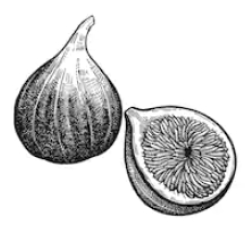
\includegraphics[width=1in,height=1.25in,clip,keepaspectratio]{fig1}}]{Michael Shell}
Use $\backslash${\tt{begin\{IEEEbiography\}}} and then for the 1st argument use $\backslash${\tt{includegraphics}} to declare and link the author photo.
Use the author name as the 3rd argument followed by the biography text.
\end{IEEEbiography}

\vspace{11pt}

\bf{If you will not include a photo:}\vspace{-33pt}
\begin{IEEEbiographynophoto}{John Doe}
Use $\backslash${\tt{begin\{IEEEbiographynophoto\}}} and the author name as the argument followed by the biography text.
\end{IEEEbiographynophoto}




\vfill

\end{document}


